\chapter{Architettura e Design}
\label{ch:architectures}

\section{Design generale del software}

L'architettura del software è basata su micro-servizi autonomi e indipendenti tra loro e la loro comunicazione avviene tramite API REST.
Esiste un middleware che si occupa della gestione e dell'orchestrazione dei micro-servizi, facendo appunto da ponte collegando le varie diverse tencologie.

I microservizi che si sono scelti di sviluppare si occupano di varie aree legate alla natura del progetto e sono:
\begin{itemize}
    % \item \textbf{ChatService}: si occupa della gestione delle chat tra utenti.
    \item \textbf{UserService}: si occupa della gestione degli utenti, quindi la loro registrazione, autenticazione e gestione dei dati personali.
    \item \textbf{BusinessLogic}: si occupa di mantenere al proprio interno tutte le regole proprie del gioco
    \item \textbf{Front-End}: si occupa di gestire l'interfaccia grafica e la comunicazione con il middleware.
    \item \textbf{Middleware}: si occupa della gestione delle comunicazioni tra i vari microservizi, e svolge la funzione di "motore di gioco".
\end{itemize}


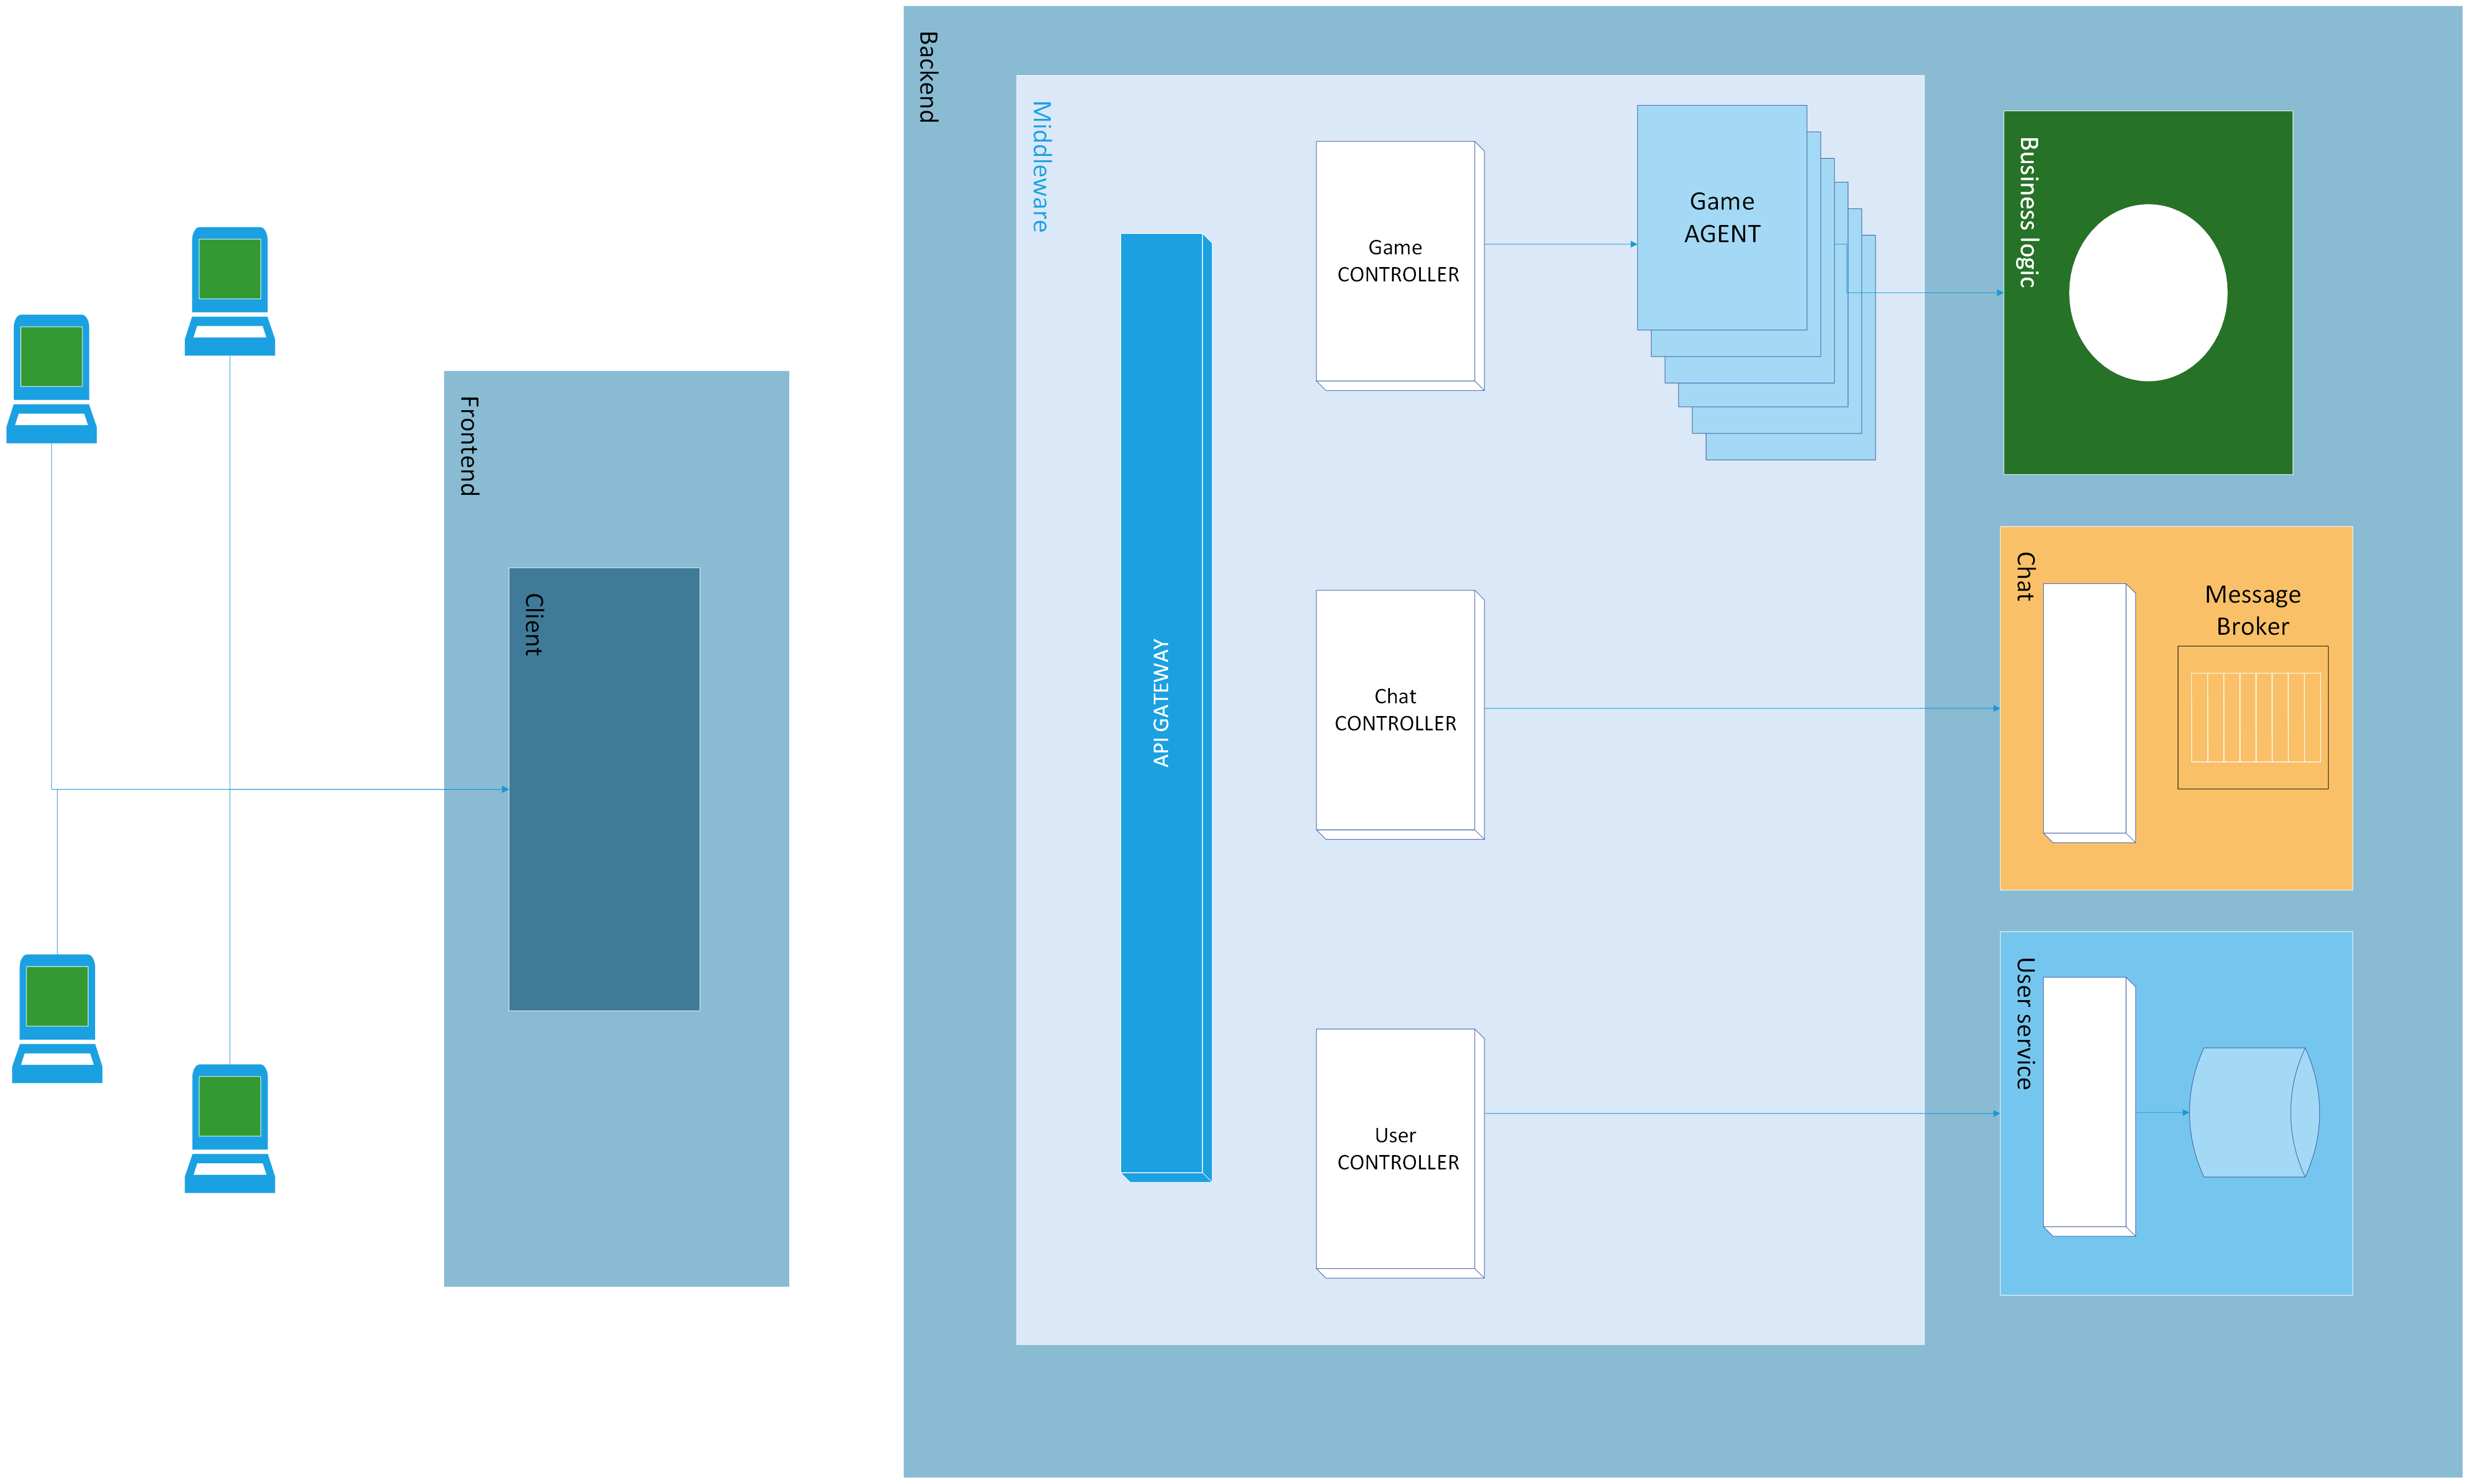
\includegraphics[width=12cm]{report/img/Architecture.png}\\[10.5cm]

Le interazioni tra i microservizi avvengono prevalentemente tramite API rest e websocket. Qui di seguito uno sequence diagram che riassume come avviene lo scambio di informazioni tra i vari componenti.

All'interno del capitolo dedicato alle Iterazioni quest'ultime verranno approfondite in dettaglio.

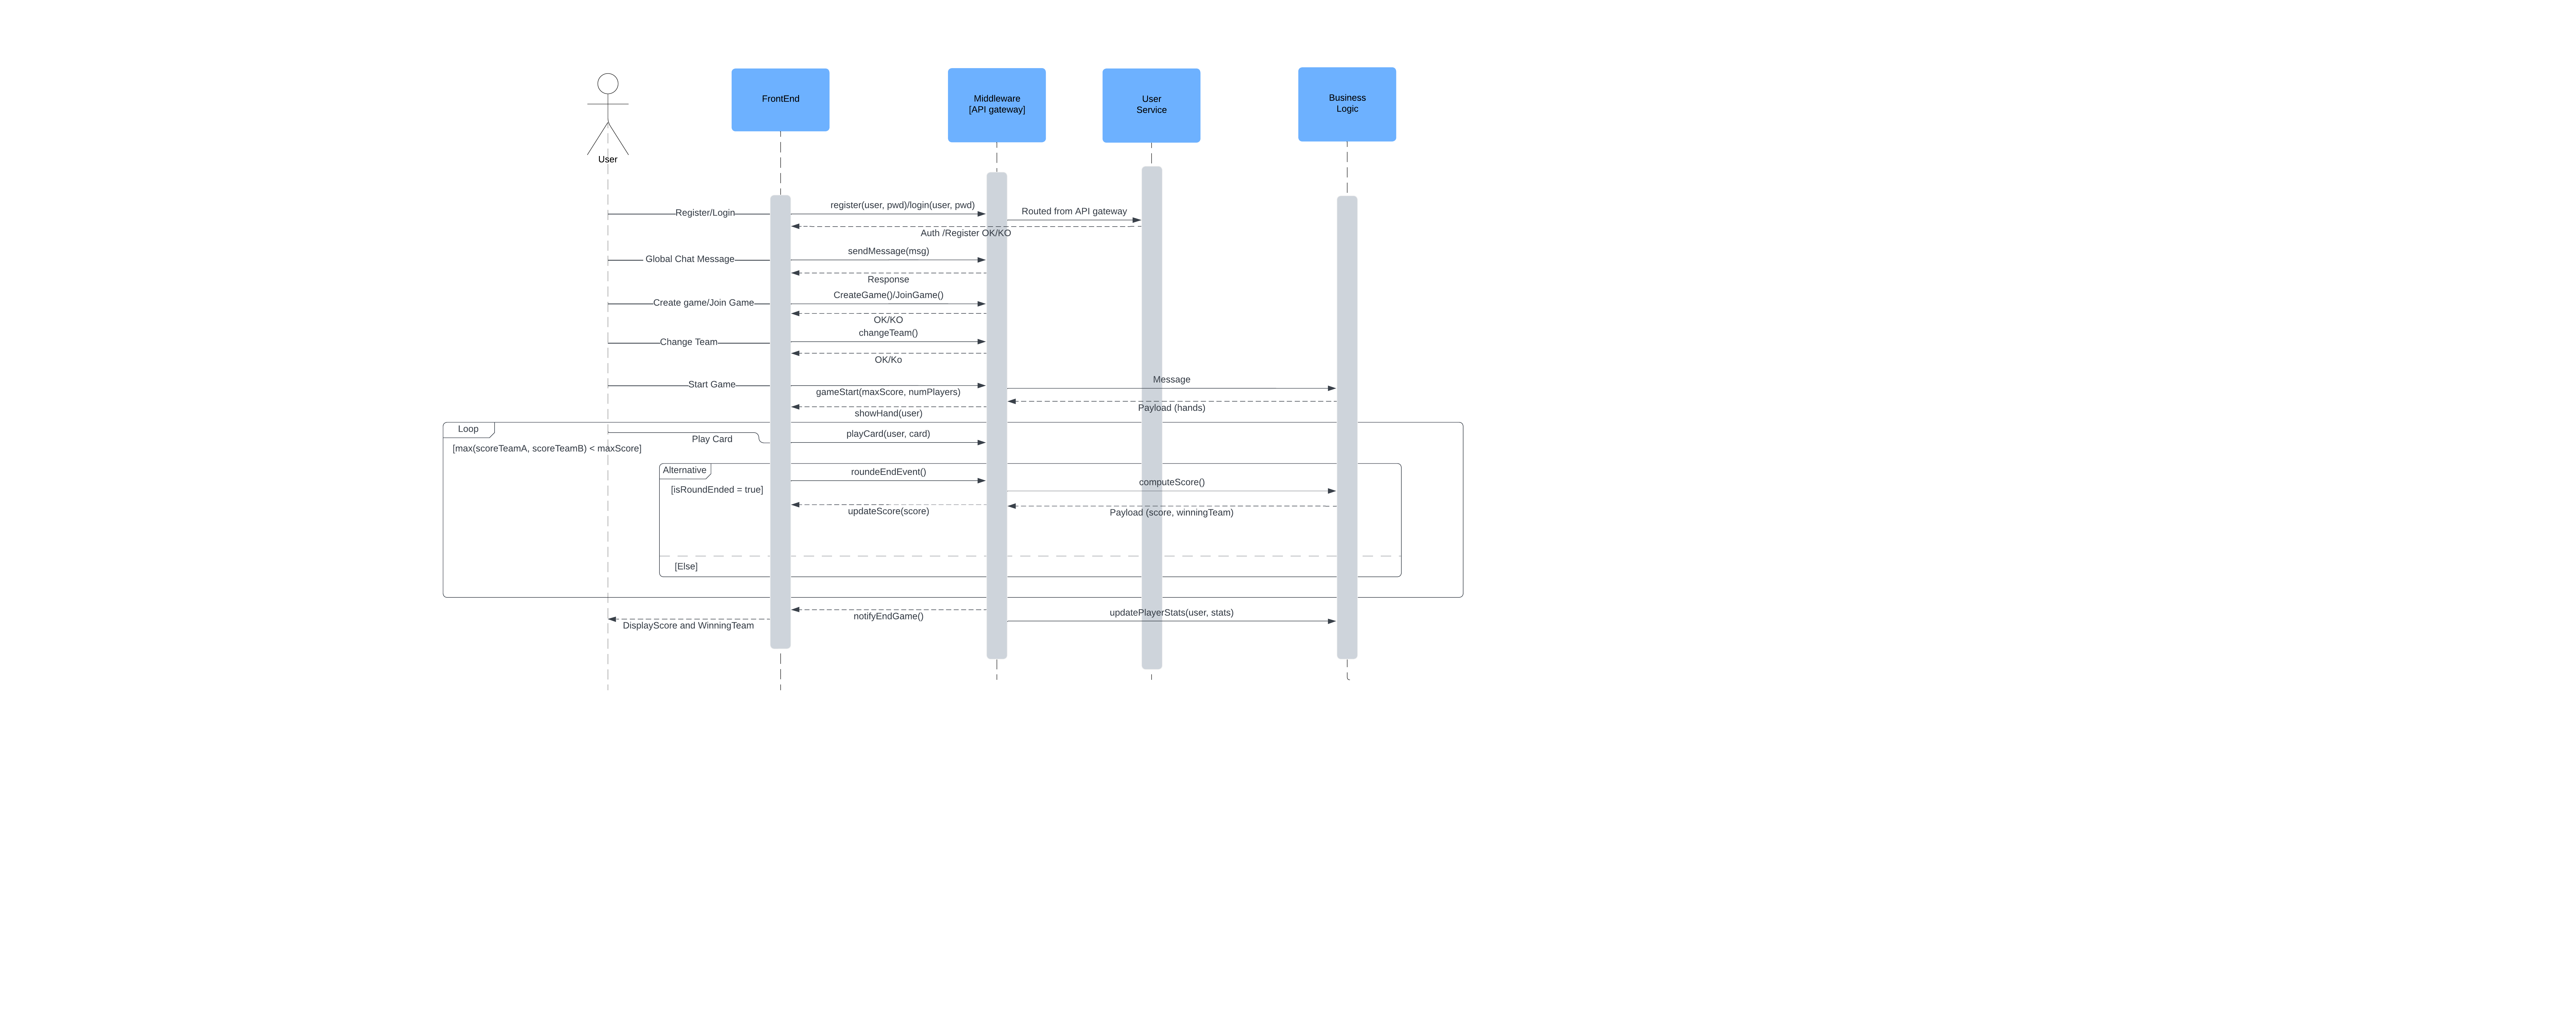
\includegraphics[width=12cm]{report/img/Maraffa_Diagram.png}\\[10.5cm]

\section{Micro-servizi e la loro architettura}

% \subsection{Servizio per la Chat}

% \begin{table}[h!]
%     \centering
%     \caption{Tabella descrittiva Chat Service}
%     \label{tab:chat_serv_table}
%     \begin{tabular}{ll}     
%         \toprule                   
%         Linguaggio & Java \\        
%         Server & Vertx, Swagger \\
%         Librerie & RabbitMQ(vertx) \\
%         Architettura & Agenti vertx \\
%         \bottomrule
%     \end{tabular}
% \end{table}

% 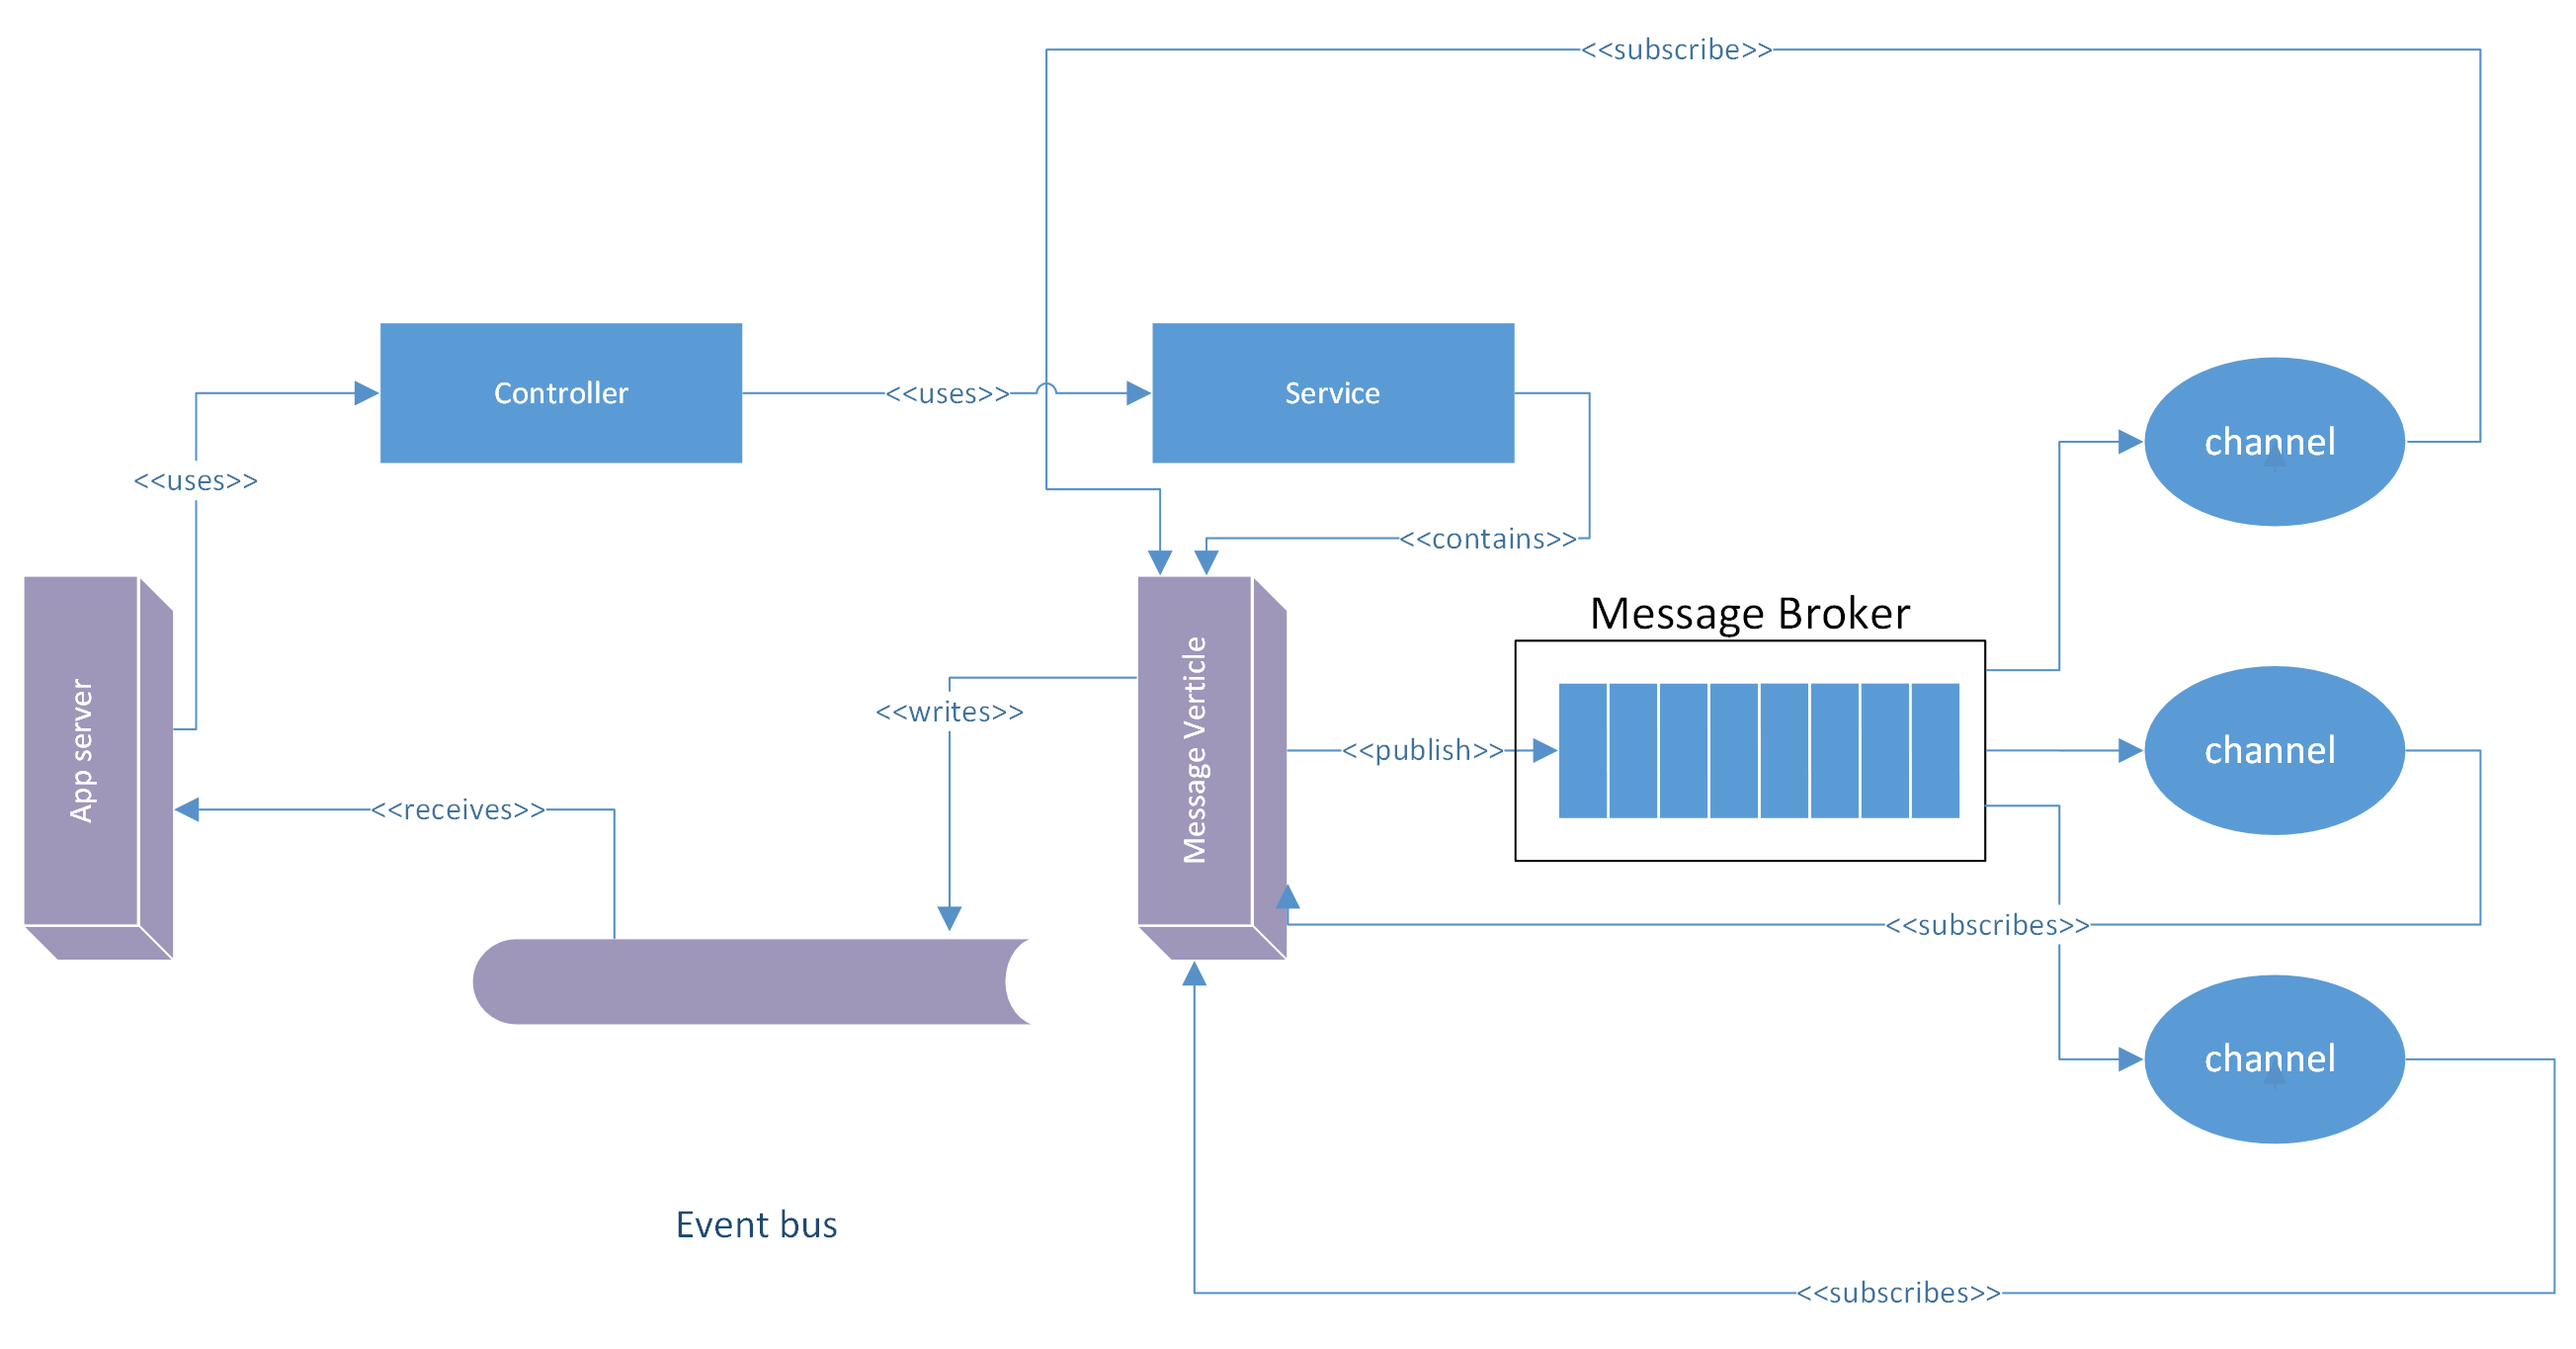
\includegraphics[width=15cm]{report/img/Architettura ChatService.png}\\[10.5cm]

\subsection{Servizio per Gestione Utenti}

\begin{table}[h!]
    \centering
    \caption{Tabella descrittiva User Service}
    \label{tab:user_serv_table}
    \begin{tabular}{ll}     
        \toprule                   
        Linguaggio & Node.JS/TypeScript \\        
        Framework & NestJS   \\                   
        Persistence & Mysql  \\
        Librerie & TypeORM   \\
        Architettura & Model-Controller-service  \\
        \bottomrule
    \end{tabular}
\end{table}


\subsection{Servizio Business Logic}

\begin{table}[h!]
    \centering
    \caption{Tabella descrittiva Business Logic}
    \label{tab:bl_serv_table}
    \begin{tabular}{ll}     
        \toprule                   
        Linguaggio & Node.JS/TypeScript \\        
        Framework & NestJS   \\                   
        Architettura & Model-Controller-service  \\
        \bottomrule
    \end{tabular}
\end{table}

\subsection{Servizio ponte tra i microservizi}


\begin{table}[h!]
    \centering
    \caption{Tabella descrittiva Middleware}
    \label{tab:middleware_serv_table}
    \begin{tabular}{ll}     
        \toprule                   
        Linguaggio & Java \\        
        Server & Vertx \\
        Librerie & RabbitMQ(vertx) \\
        Architettura & Multi-agent, motore di gioco \\
        \bottomrule
    \end{tabular}
\end{table}

\section{Perche' i microservizi?}

Ogni microservizio si occupa di gestire un singolo ambito di progetto, il che fa sì che si ottengano ottimi risultati riguardo la qualità e l'affidabilità, la riutilizzabilità, la flessibilità e la scalabilità.
Tutti i componenti sono "loosely coupled", distribuiti in modo indipendente, altamente collaudabili e gestibili e in ambiti reali gestiti da un piccolo team.
Tuttavia, non si tratta di una soluzione definitiva, ha anche degli svantaggi come ad esempio:
\begin{itemize}
    \item la complessità di gestione e la necessità di un'infrastruttura di rete molto complessa.
    \item un'ottima comunicazione di team.
    \item una discreta capacità di astrazione e progettazione di interfaccie di comunicazione che devono essere rispettate da tutti i microservizi.
    \item Non si ha la certezza che l'infrastruttura funzioni correttamente fino a quando tutti i servizi non cooperano tra loro.
\end{itemize}

% \subsection{[SPE] Vantaggi}
% - devops
% - ci 

\subsection{Vantaggi dell'architettura a microservizi}

\subsubsection{Fault Tolerance}

Progettare un sistema completamente privo di errori è un obiettivo decisamente ambizioso e molto difficile da raggiungere. 
Molto più realistico, e inerente al nostro percorso, è progettare un sistema che sia in grado di tollerare, nella giusta misura, gli errori che inevitabilmente si verificheranno. 
La scelta di questa architettura tra i vari vantaggi offre la possibilità di \textbf{isolare parti del sistema}, evitando che gli errori si propaghino in modo incontrollato e che il sistema nel suo complesso vada in crash. 
Ogni sistema opera in modo indipendente e autonomo, con le proprie risorse e la propria logica.
\vspace{1cm}

Lo snodo centrale di comunicazione dei servizi, il middleware, è in grado di gestire le comunicazioni tra i vari microservizi e di garantire che il sistema sia in grado di funzionare anche in caso di guasti.
Purtroppo non esiste alcun progetto senza alcun tipo di \textbf{single point of failure}, o almeno non con le risorse a disposizione di noi studenti, quindi all'interno di questo servizio la 
gestione degli errori dei servizi con cui comunica è gestita, ma di fatto, nel caso in cui il middleware smetta di funzionare, non avendo nessun altro servizio che possa fare da garante 
per il suo corretto funzionamento, tutto il sistema non permetterà, ad esempio, di giocare a nessun gioco.
Questo perché il middleware è il cuore pulsante del sistema; avendo disponibilità di risorse e abbastanza conoscenze in un ambito reale, questo problema ha soluzioni: 
\begin{itemize}
    \item \textbf{Backup del middleware}: avere dei backup dei processi che si occupano di gestire le partite, ma questo significherebbe andare a modificare inevitabilmente 
    la struttura già esistente del servizio.
    \item \textbf{Ridondanza del middleware}: avere molteplici istanze del middleware, preferibilmente 3, di cui una principale e le altre 2 in copia, facendo in modo che
    ogni azione sul middleware principale venga replicata sulle altre due istanze e che quindi, in caso di guasto hardware, le altre copie possano rispondere alle richieste.
    Se si utilizza questa soluzione bisogna prestare attenzione alla consistenza delle copie. La non consistenza potrebbe addirittura peggiorare la situazione.
    Per questo motivo è consigliato averne più di una, in modo tale da controllarne la consistenza.
\end{itemize}

\subsubsection{Scalabilità}

Nel caso del middleware, la scalabilità è un altro modo per chiamare la duplicazione, ma questo si applica soltanto al middleware, in quanto gli altri microservizi sono realmente scalabili.
Ogni microservizio è in grado di scalare in modo indipendente, in base alle proprie esigenze, e questo permette di avere un sistema che si adatta in modo dinamico alle richieste degli utenti. 
Nella prossima sezione verrà approfondito come il deployment con Docker permetta di scalare i microservizi. L'implementazione di un sistema di load balancing viene fornita
"gratuitamente" da Kubernetes, che permette di bilanciare il carico tra i vari nodi del cluster. 
Qualora il progetto maraffa-online dovesse avere un numero di utenti molto elevato, si potrebbe pensare di scalare il sistema in modo orizzontale, aggiungendo nuovi nodi al cluster, 
e tramite la dovuta configurazione, Kubernetes si occuperebbe di bilanciare il carico tra i vari nodi dei servizi scalabili. 


\subsubsection{Docker}

Suddividere un progetto monolitico in servizi a sé stanti permette di dockerizzare comodamente ogni servizio e questo consente di avere un sistema facilmente deployabile, versionabile e portabile.
Uno dei requisiti fondamentali del progetto era riuscire a dockerizzare interamente il sistema. Nel caso in cui si volesse fare un deploy su un server remoto, sarebbe sufficiente avere Docker installato, accedere al docker-compose del progetto, settare le corrette variabili d'ambiente e poi il progetto opererebbe in totale autonomia.
Inoltre, utilizzare uno stack permette anche di gestire eventuali failure dei servizi in modo più semplice, poiché Docker consente di avere un sistema fault-tolerant. Se un servizio dovesse andare in crash per qualche motivo inspiegabile, Docker si occuperebbe di riavviarlo in modo autonomo.
L'utilizzo di uno stack permette anche di scalare i servizi in modo più semplice, poiché basta settare il numero di repliche desiderate per un servizio e Docker si occuperà di creare le repliche e di bilanciare il carico tra di esse. Questo è un vantaggio nel caso in cui si voglia scalare il sistema in modo orizzontale, ovvero aumentando le instanze di un singolo servizio.


\subsection{Struttura API Gateway}

Il pattern di progettazione utilizzato per la realizzazione del middleware è quello dell'API Gateway, che permette di creare un'interfaccia unica per l'accesso ai vari servizi del sistema.

Nel nostro progetto, il client effettua semplici chiamate verso il middleware, che nei casi necessari effettua chiamate verso altri servizi per svolgere una determinata operazione.
Queste chiamate non sono obbligatoriamente dirette verso il servizio interessato, ma possono anche essere routine che effettuano molteplici chiamate per ottenere il risultato desiderato. 
Implementare queste chiamate direttamente nel front-end avrebbe reso il codice molto più complesso e difficile da mantenere, e la gestione di partite multiple sarebbe stata molto più difficile.

\vspace{1cm}

Non è stato implementato nessun meccanismo di discovery per la gestione di chiamate verso gli altri servizi, in quanto tutti presenti sullo stesso server e nello stesso stack di Docker, quindi facilmente individuabili sulla rete virtuale creata da Docker.

\vspace{1cm}

Si è seguito un approccio modulare nello sviluppo di questo componente che, in un primo step, conteneva soltanto la logica di gestione delle partite, al quale sono stati aggiunti i moduli per la comunicazione con il servizio degli utenti e della business logic. Ogni modulo segue la stessa struttura, ossia una classe denominata controller che si occupa esclusivamente della dichiarazione delle rotte HTTP e che a sua volta contiene un service. Ogni servizio contiene poi le logiche di calcolo e crea un JSON di risposta che viene passato al controller che lo invia come risposta HTTP, questo per poter separare completamente e rispettare il principio di single responsibility.

Nel modulo contenente le logiche di gioco è stato necessario aggiungere un ulteriore strato alla struttura controller-service, data la struttura multi-agente della gestione delle partite che non permetteva una separazione netta. Quindi è stato aggiunto, tra il controller e il service, un componente ibrido per poter comunque avere servizi indipendenti.

Questa separazione, oltre a essere una buona pratica, è stata scelta per poter effettuare del testing comodamente soltanto sui servizi, testando quindi solamente la parte relativa all'elaborazione di una risposta.

\subsection{WebSockets}

L'interazione con il frontend avviene prevalentemente tramite il protocollo HTTP, ma per la gestione di alcuni aspetti in tempo reale sono state introdotte le WebSocket.
Questo componente è stato creato, ad esempio, per la gestione delle chat di gioco, in modo che i giocatori possano comunicare tra loro in tempo reale. Ogni client, istanziato sul computer degli utenti, effettua una connessione WebSocket con il middleware utilizzando come endpoint il proprio UUID, che viene assegnato automaticamente all'avvio, e lo username del giocatore, dopo aver effettuato il login. Il middleware contiene al proprio interno una mappa di tutti i client e giocatori connessi con la relativa WebSocket e una classe che espone due metodi per inviare messaggi a un singolo giocatore o effettuare un messaggio broadcast a tutti i giocatori connessi.

Il modulo di game si occupa di gestire le partite, quindi è l'unico che può sapere quali giocatori devono ricevere determinati messaggi relativi a una singola partita. Per utilizzare il servizio di WebSocket, è stata implementata una semplice interfaccia all'interno dell'agente di gioco con la quale si effettuano chiamate "onEvent". Ogni volta che un particolare evento si verifica, un'invocazione a queste chiamate permette di inviare messaggi alle WebSocket dei giocatori interessati.

\begin{lstlisting}[language=Java, caption={Interfaccia per gestire chiamate websocket}, label=list:java_websocket_interface]
package game;

import game.service.User;

public interface IGameAgent {

	void onCreateGame(User user);

	void onNewRound();

	void onJoinGame(User user);

	void onStartGame();

	void onCheckMaraffa(int suit, String username);

	void onPlayCard();

	void onTrickCompleted(Trick latestTrick);

	void onMessage();

	void onEndRound();

	void onEndGame();

	void onNewGame(String newGameID);

	void onChangeTeam();

	void onMakeCall(final Call call);
}
\end{lstlisting}

% \section{Punti comuni tra i servizi}

% \subsection{Swagger}